\begin{Schunk}
% --begin: "horizon"
\begin{Sinput}
R> ctx <- ctx3()
R> sm <- horizon(ctx, atomic = "sm")
R> me <- horizon(ctx, atomic = "me")
R> bi <- horizon(ctx, atomic = "bi")
R> g <- ggplot(data = data.frame(x = 0), mapping = aes(x = x))
R> g + stat_function(aes(color = "sm"), fun = sm) + stat_function(aes(color = "me"), 
+     fun = me) + stat_function(aes(color = "bi"), fun = bi) + xlim(-0.5, 1.5)
\end{Sinput}

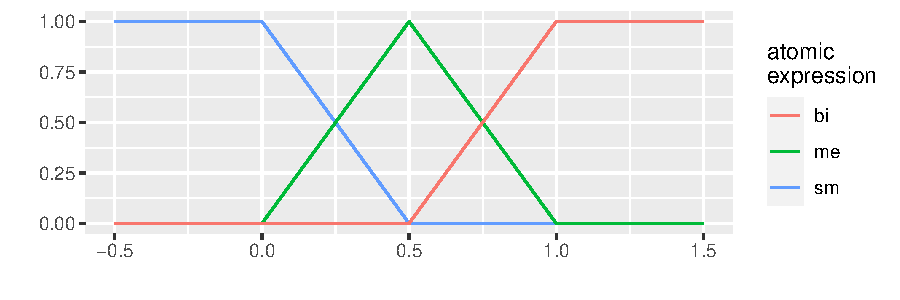
\includegraphics[width=\maxwidth]{figure/unnamed-chunk-12-1} %
% --end: "horizon"
\end{Schunk}
